\chapter{实验验证}

\section{实验配置及关键问题}

在整个实验验证的过程中,我们实验使用的机器使用了Ubuntu 18.04 bionic系统,配置了8$\times$2核 2.10GHz的英特尔Xeon E5-2620V4处理器,32 GB内存和4 TB的机械硬盘。对于我们在实验过程中使用的分析工具,我们全部使用默认配置,也没有使用多线程技术。

在实验过程中,我们使用几种分析工具的最新版本进行漏洞签名的归纳总结,并在26354个合约的学习数据集上完成了对安全盾技术的总结。为了获取学习数据集,我们实现了一个网络爬虫,这个爬虫可以从Etherscan,一个著名的第三方区块分析服务提供站上面爬取Solidity源代码。在我们爬虫指出,Etherscan没有限制用户自由下载Solidity代码,但是到2019年年初,Etherscan限制每个用户只能查看最新的1000个经过验证的合约代码,而不能查看以往的合约代码。最终,我们借助最初爬取的26354个智能合约进行标准漏洞库的构建。在爬虫过程中,爬虫使用了随机的搜索策略以保证我们从Etherscan下载的Solidity源代码是随机的。

对于我们用于验证工具的数据集,鉴于我们从26354个合约上观察总结了安全盾技术,如果再把这些数据集用于工具的验证,会显得不够公平。因此,我们从Google BigQuery Open Dataset上爬取了一系列的合约地址,再经过从Etherscan上获取合约源代码,我们最终得到了11516个部署在以太坊之上的真实Solidity代码。在这个数据集上我们能够公正地进行我们的检测系统的验证工作,并和其他工具做比较。至于在验证环节用到的各个分析工具,我们皆采用当前能获取到的最新版本:Slither v0.6.4,Oyente v0.2.7,Smartcheck v2.0和Securify v1.0。

在本章,我们希望围绕三个关键问题(Research Questions)来阐述和分析实验:
\begin{itemize}
  \item[\textbf{RQ1}] 构建的标准漏洞库质量如何?这些提取的签名真的具有代表性吗?发现的漏洞有效吗?
  \item[\textbf{RQ2}] 我们构建的检测系统准确率如何?对比其他检测工具是怎样的结果?
  \item[\textbf{RQ3}] 我们系统在构建标准漏洞库的过程中和对比其他工具的过程中的效率如何?
\end{itemize}

\section{RQ1:验证漏洞签名以及构建的标准漏洞库}

在我们漏洞签名以及安全盾技术应用于寻找漏洞的过程中,我们通过找到的漏洞不断反馈修缮漏洞签名,使得最终获得的漏洞签名也是我们成果的一部分,进而我们能借助漏洞签名和安全盾技术找到更多的漏洞。最终,我们分析了所有工具报告的真实漏洞样本,在此基础上我们构建了标准漏洞库。

\subsection{分析收集具有代表性的漏洞签名}

基于各个工具的源代码、论文以及他们所报告的真实漏洞,我们分析总结出了漏洞签名。因为我们主要通过开源的仓库,已经发表的论文等获取分析工具的特点,在一些漏洞签名上我们无法做到完全理解,由此造成了获取的漏洞签名没有完整体现工具的特点,我么通过观察各工具对漏洞的报告情况不断调整签名。同时,为了保证提取的漏洞签名具有一定程度的代表性,我们将部分包含漏洞的代码使用树的编辑距离算法\cite{treeEditDistance}计算,并进行聚类,最后再将聚类后得到的代码的共同特征进行抽象,再和我们的漏洞签名进行比对,这样使得我们总结的漏洞签名不仅代表了前沿分析工具的技术结晶,也代表了真实漏洞的代码的核心成分。

\subsection{不同工具发现的漏洞分布}

为了辨认现有工具报告的漏洞,一些人为的审计是无法避免的。但我们采取了一些策略来加速这个人工审计的过程,同时也保证了审计具有一定的准确度。例如,如果一段代码被\textsc{Slither}、\textsc{Oyente}、\textsc{Smartcheck}和\textsc{Securify}中两个或两个以上的工具报告为漏洞,我们觉得这段代码具有较高的可信度,因此指派一名领域专家对这段代码进行审计;否则如果一段代码只被一个工具报告为漏洞,我们会指定两名领域专家对这段代码进行审计,如果这两名领域专家的意见相反,我们会指定第三名领域专家介入并做最终判断。在获取了以上工具报告的所有真实漏洞后,我们才能构建一个对漏洞准确率具有较高置信度的标准漏洞库。
\begin{figure}
  \centering
  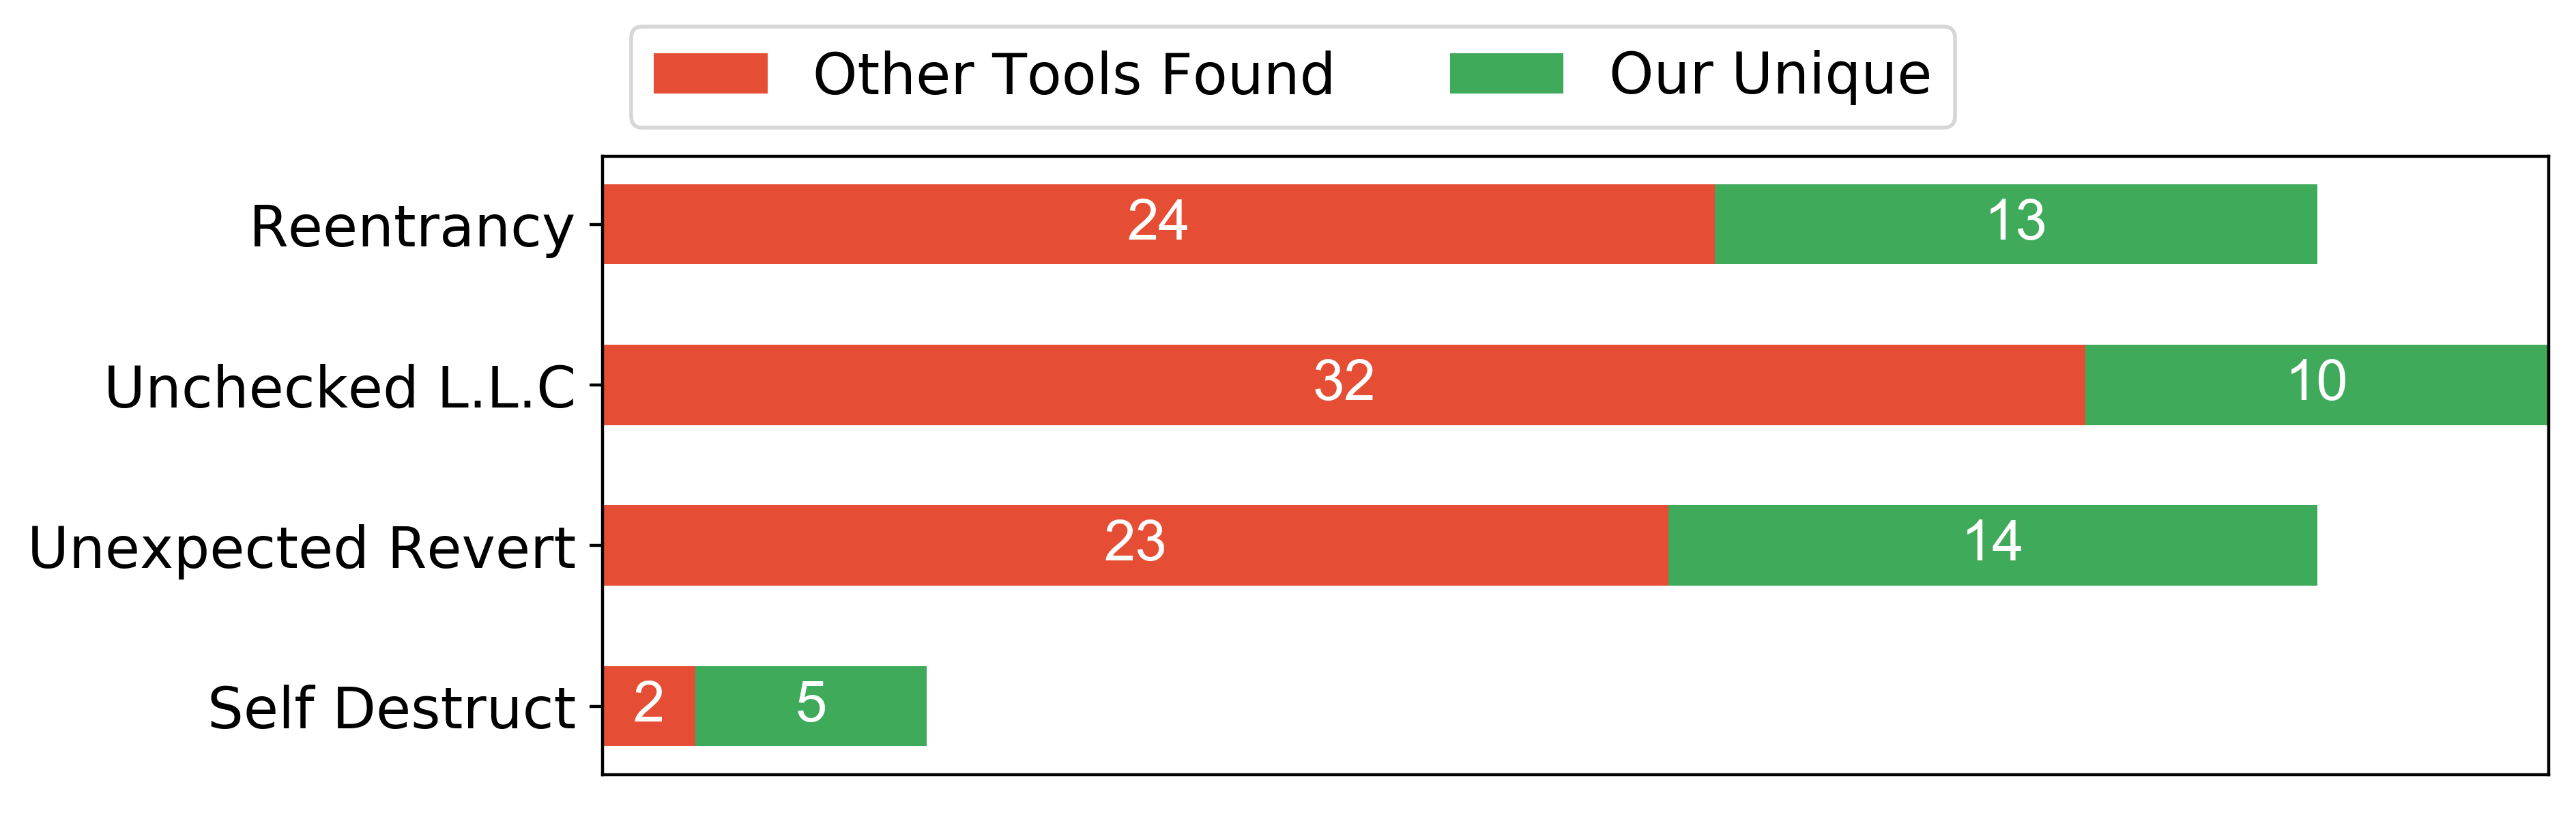
\includegraphics[width=\linewidth]{figures/unique_tp.png}
  \caption{发现的真实漏洞数量统计,“Our Unique”表示只被我们发现的漏洞}\label{fig:unique_tp}
\end{figure}
如图所示,这个标准漏洞库包含了123个漏洞实例。在这之中,可重入漏洞和低级调用漏洞占了所有漏洞数量可观的比重,其他两个漏洞则较少。在实验完成之后并联系上漏洞关联软件的开发者后,我们会将部分漏洞在网站上进行公开。

\subsection{动态验证漏洞的真实性}

为了验证我们在实验中检测到的漏洞的真实性,我们对漏洞实例进行了简单的随机采样,并试图在我们的本地环境进行漏洞的触发。特别地,我们针对每个漏洞签名采样2个漏洞进行测试,只选用两个漏洞是因为使用漏洞签名匹配的可疑代码大多相似,如果测试代码被成功出发,则这些相似的代码也能用类似的测试方式进行触发;还有个原因是每次测试所需要的测试用例都需要我们的领域专家进行独立设计,如果需要进行测试的实例太多,会有大量的时间消耗。测试的环境采用了\textsc{Remix}本地环境进行测试。至于如何使用自动化流程进行软件代码测试,或者如何保证测试的高效性和有效性,这些问题超出了本课题研究的范围,不作讨论。

\section{RQ2:分析各检测系统的检测结果}

在上一章第\ref{sec:detection_rules}节和第\ref{sec:ss}节中,我们讨论了漏洞签名的归纳总结过程和9中安全盾技术的特点。为了分析这些漏洞签名和安全盾的有效性,我们将11516个未使用的智能合约软件用作测试集,在测试集上使用各种前沿工具以及我们的检测系统进行实验,最后比对检测结果。在统计时,我们将每个工具报告的漏洞都经过了人工专家的审计,这使得我们认为的漏洞代码数据是具备一定可信度的。各个工具在各个漏洞上的检测准确率如表\ref{tab:eval_reentrancy}、\ref{tab:eval_revert}、\ref{tab:eval_llc}、\ref{tab:eval_selfdestruct}所示。

\begin{table}[htbp]
  \centering
  \begin{minipage}[t]{0.48\textwidth}
  \caption{可重入漏洞检测结果}
    \begin{tabular}{cccc}
    \toprule
    Tools & \#N & P\% & R\% \\
    \midrule
    Slither & 79    & 18.98\%  & 40.54\% \\
    Oyente & 19  & 10.53\%     & 5.40\% \\
    Smartcheck  & $\times$     & $\times$  & $\times$  \\
    Securify &  261    & 4.59\%  & 32.43\% \\
    Athena & 58   & 27.59\%     & 43.24\% \\
    \bottomrule
    \end{tabular}%
  \label{tab:eval_reentrancy}%
  \end{minipage}
  \begin{minipage}[t]{0.48\textwidth}
    \caption{意外异常漏洞检测结果}
    \begin{tabular}{cccc}
    \toprule
    Tools & \#N & P\% & R\% \\
    \midrule
    Slither  & 137  & 10.95\%   & 51.35\% \\
    Oyente  & $\times$ & $\times$  & $\times$ \\
    Smartcheck  & 29  & 65.52\%   & 40.54\% \\
    Securify  & $\times$  & $\times$  & $\times$ \\
    Athena & 43   & 79.07\%     & 91.89\% \\
    \bottomrule
    \end{tabular}%
  \label{tab:eval_revert}%
  \end{minipage}
  \begin{minipage}[t]{0.48\textwidth}
    \caption{低级调用漏洞检测结果}
    \begin{tabular}{cccc}
    \toprule
    Tools & \#N & P\% & R\% \\
    \midrule
    Slither & 18   & 100.0\%     & 42.86\% \\
    Oyente  & $\times$ & $\times$ & $\times$ \\
    Smartcheck  & 91     & 45.05\%     & 52.38\% \\
    Securify & $\times$ & $\times$ & $\times$ \\
    Athena &  38  & 89.47\%    & 80.95\% \\
    \bottomrule
    \end{tabular}%
  \label{tab:eval_llc}%
  \end{minipage}
  \begin{minipage}[t]{0.48\textwidth}
    \caption{自毁漏洞检测结果}
    \begin{tabular}{cccc}
    \toprule
    Tools & \#N & P\% & R\% \\
    \midrule
    Slither & 10    & 20.00\%    & 28.57\% \\
    Oyente  & $\times$ & $\times$ & $\times$ \\
    Smartcheck  & $\times$ & $\times$ & $\times$ \\
    Securify & $\times$  & $\times$ & $\times$ \\
    Athena & 30    & 23.33\%     & 100.0\% \\
    \bottomrule
    \end{tabular}%
  \label{tab:eval_selfdestruct}%
  \end{minipage}
    \label{tab:eval_all}
\end{table}%

表中的"\#N"表示工具报告漏洞的数量,"P\%"和"R\%"分别表示了精确率和覆盖率,其中精确率的计算方式为(该工具报告的TP数)/\#N,覆盖率的计算方式为(该工具报告的TP数)/(所有工具的TP集合) 。下面我们将对表格中数据做简单的总结,并对数据背后的原因做简单分析。

\subsection{Athena产生误报的原因}

在表\ref{tab:eval_reentrancy}、\ref{tab:eval_revert}、\ref{tab:eval_llc}、\ref{tab:eval_selfdestruct}中,我们列举了91个由\textsc{Athena}找到的漏洞,不考虑漏洞的类型,\textsc{Athena}有着53.84\%的总体精确率。相比之下,\textsc{Slither}具有着20.49\%的总体精确率,\textsc{Oyente}有着10.53\%的总体精确率,\textsc{Smartcheck}具有着40.59\%的总体精确率, \textsc{Securify}有着4.59\%的总体精确率。以上的精确率是建立在第\ref{sec:detection_rules}节中引入的漏洞签名和在第\ref{sec:ss}中引入的安全盾技术的基础上进行统计和整理的。

\subsubsection{可重入漏洞误报的原因}

在四个支持检测可重入漏洞的工具中,\textsc{Athena}有着最低的误报率(准确率27.53\%),这是因为我们采用了SS1-5的安全盾技术,针对可重入漏洞的检测做出改进,有效降低了在可重入漏洞上的误报率。其他工具的误报率都要高于甚至显著高于我们的系统。例如,\textsc{Securify}的误报率高达95.41\%,这是因为它的检测规则过于宽泛和简单,而且没有考虑代码中的安全盾技术。\textsc{Slither}的检测规则比较严谨和规范,但是它同样不考虑安全盾技术,这导致它虽然有着可接受的覆盖率40.54\%,准确率却比较低18.98\%。\textsc{Oyente}同样没考虑安全盾技术的存在,由于它的规则过于严格,它的覆盖率5.40\%较低,但准确率10.53\%较高。

\subsubsection{意外异常漏洞误报的原因}

正如在第\ref{sec:detection_rules}节归纳的一样,Slither将在循环结构中的所有调用都判作漏洞,这导致了它122个误报。Smartcheck在检测时考虑了SS6但是没有考虑SS7。相比之下,\textsc{Athena}考虑了SS6与SS7,这使得我们的系统产生的误报数量更少。

\subsubsection{低级调用漏洞误报的原因}

Slither在这个漏洞上的精确度表现很好,没有一个误报,这是因为它严格地检查了三种低级调用,\codeff{call}、\codeff{delegatecall}、\codeff{send}的使用。Smartcheck没有考虑SS8,因此报告了很多高级调用,导致了50个误报。Athena有4个误报,这几个误报的原因是因为在函数中这些低级调用的返回值在其他语句受到了检查,而不是直接低级调用写在一起。因此,这4个误报需要借助数据依赖分析去寻找它被检查的位置。

\subsubsection{自毁漏洞误报的原因}

在这个漏洞上Athena有24个误报,在观察误报的原因之后,我们发现这些误报的原因是出自于复杂的函数修饰器,这些函数修饰器将身份检查功能隐藏于调用链中,无法直接准确分析。Slither有着接近的精确率,并报告了8个FP。

\subsubsection{小结}

我们总结的安全盾技术能在多数类型的漏洞中减少误报的数量。可是,SS3、SS9这两种安全盾的总结还不够令人满意,在遇到复杂的用户自定义函数修饰器或者是许多本地变量的使用时的表现不尽人意。要解决以上问题,必须进一步地采用数据依赖分析技术进行辅助。

\subsection{Athena具有高覆盖率的原因}

在表\ref{tab:eval_reentrancy}、\ref{tab:eval_revert}、\ref{tab:eval_llc}、\ref{tab:eval_selfdestruct}中,Athena具有着最好的覆盖率表现,在四种漏洞上的表现都要好于或者远好于其他工具。

\subsubsection{可重入漏洞真实漏洞的分布}

Athena找到了13个其他工具都没有发现的漏洞,我们观察这13个漏洞之后认为,其他的三个工具都没能考虑用户自定义的\codeff{transfer}函数,只考虑了Solidity内建的\codeff{transfer}函数。另外,Athena漏掉了34个真实漏洞,很显然这是因为可重入漏洞的复杂超过我们的预计,我们的漏洞签名仍然没能充分包括这部分真实漏洞。

\subsubsection{意外异常真实漏洞的分布}

对于这个漏洞类型,共有5个真实漏洞是只被一种工具唯一发现的,其中有2个是被Athena发现的。有趣的是,大部分的该类型的真实漏洞是被至少两种工具发现的——这说明其他工具的检测规则和我们的漏洞签名相似。其他3个只被一种工具唯一发现的漏洞没有在Athena的报告范围内,这是因为这些代码使用\codeff{assert}检查循环结构中的\codeff{transfer}语句,这也会造成意外异常漏洞,且不在我们漏洞签名的考虑范围内。

\subsubsection{低级调用真实漏洞的分布}

在18个只被一种工具唯一发现的真实漏洞中,Athena发现了10个,这10个里低级调用被\codeff{if}的条件语句使用,但是没有在\codeff{if}语句中进行检查,因此不会被报告为真实漏洞。Athena漏洞签名去尽可能匹配疑似漏洞的数据集。可是,仍有8个漏洞被Athena漏掉了。在观察这8个漏洞之后,我们发现这8个漏洞的低级调用的返回值赋值给了别的变量,对于变量的检查在后面的语句中产生,这是种非直接检查的低级调用。由于我们并没有在系统中加入数据依赖分析,Athena没能将这类代码报告为漏洞。Slither、Smartcheck将这8个报告为漏洞的原因是因为这些低级调用存在于\codeff{if}结构的条件语句内。

\subsubsection{自毁漏洞真实漏洞的分布}

对于这类漏洞,Athena报告了5个唯一发现的真实漏洞,并有着出众的覆盖率表现。我们自毁漏洞的漏洞签名较㢖,也考虑了用户自定义的函数修饰器,综合影响之下,覆盖率远好于Slither的28.57\%。同时,高覆盖率也带来了较低的准确率,Athena的准确率稍高于Slither。

\subsubsection{小结}

基于观察各前沿工具的实现原理和阅读大量代码得到的四种漏洞签名,只被Athena检测出的漏洞数要远高于其他工具检测出的数量。在检测低级调用漏洞时,Athena仍需要再加入准确的数据依赖分析,以提高系统的覆盖率表现。

\section{RQ3:验证系统的运行效率}

在表\ref{tab:time_cost}中,Slither仅消耗了52分钟就完成了检测工作。而Smartcheck和Athena这两个工具采用了相近的核心技术——基于规则的静态分析,因此本应具有相近的运行时间 (0~500 min)。实际上,由于实现的差异,两种工具的运行时间有一定的差距,但这两个工具的检测速度仍然原快于Oyente和Securify,因为他们使用了约束求解技术,增加了时间的消耗。值得一提的是,我们提取漏洞签名的时间,包括安全盾技术的加入,没有被包含在整个系统的运行时间内。

\begin{table}
  \centering
  \caption{各工具的检测时间,单位为分(min)}
  \begin{tabular}{cccccc}
    \toprule
    % after \\: \hline or \cline{col1-col2} \cline{col3-col4} ...
    Contracts & Slither & \textsc{Oyente} & Smartcheck & Securify & Athena \\
    \midrule
    11516 & 52 & 1081 & 112 & 6201 & 236 \\
    \bottomrule
  \end{tabular}
  \label{tab:time_cost}
\end{table}

从检测速度上来说,Slither是效率最高的工具,Oyente是除Securify之外效率较高的工具,Athena和Smartcheck具有较高的效率。如果考虑系统的准确率、覆盖率等综合因素,Athena是所有工具中最突出的。